\documentclass[a4paper]{book}

\usepackage{draftwatermark}
\SetWatermarkText{Draft}
\SetWatermarkColor[gray]{0.9}

\usepackage[utf8]{inputenc}
\usepackage[T1]{fontenc}

\usepackage{titlesec, blindtext, xcolor}
\definecolor{gray75}{gray}{0.75}
\definecolor{base00}{HTML}{fafafa}
\definecolor{base01}{HTML}{d4d4d4}
\definecolor{base02}{HTML}{abacae}
\definecolor{base03}{HTML}{7e8087}
\definecolor{base04}{HTML}{555761}
\definecolor{base05}{HTML}{333333}
\definecolor{base06}{HTML}{4d4d4d}
\definecolor{base07}{HTML}{666666}
\definecolor{base08}{HTML}{a10705}
\definecolor{base09}{HTML}{0d52bf}
\definecolor{base0A}{HTML}{cc3b02}
\definecolor{base0B}{HTML}{57392d}
\definecolor{base0C}{HTML}{d48e15}
\definecolor{base0D}{HTML}{3a9104}
\definecolor{base0E}{HTML}{7239b3}
\definecolor{base0F}{HTML}{667885}

\newcommand{\hsp}{\hspace{10pt}}
\titleformat{\chapter}[hang]{\Huge\bfseries}{\textcolor{base02}{\thechapter }\hsp}{0pt}{\Huge\bfseries}
\titleformat{\section}[hang]{\Large\bfseries}{\textcolor{base01}{\thesection}\hsp}{0pt}{\Large\bfseries}
\titleformat{\subsection}[hang]{\large\bfseries}{\textcolor{base01}{\thesubsection}\hsp}{0pt}{\large\bfseries}

\usepackage[american]{babel}
\usepackage{csquotes}
\usepackage[style=apa,sortcites=true,sorting=nyt,backend=biber]{biblatex}
\DeclareLanguageMapping{american}{american-apa}
\addbibresource{references.bib}

% Essentials
\usepackage{tabularx}
\usepackage{supertabular}
\usepackage{graphicx}
\usepackage{subcaption}
\usepackage[ruled]{algorithm2e}

% Typography
\usepackage{palatino}
\usepackage{fontenc}

% Links
\usepackage[colorlinks=true, citecolor=base08, linkcolor=base08, urlcolor=base08]{hyperref}

% Math stuff
\usepackage{amsmath}
\usepackage{amssymb}
\usepackage{amstext}
\usepackage{bm}

% Drawings
\usepackage{tikz}
\usetikzlibrary{arrows.meta, fit, positioning, shapes}
\newcommand{\empt}[2]{$#1^{\langle #2 \rangle}$}

\tikzset{
    neuron/.style={
        circle, draw, thick,
        inner sep=0pt,
        minimum size=3.0em,
        node distance=4em
    },
    io/.style={
        neuron,
        fill=base01
    },
    conn/.style={
        thick,
        -{Straight Barb[angle=60:2pt 3]},
    },
    connl/.style={
        thick,
        {Straight Barb[angle=60:2pt 3]}-,
    },
    prod/.style={circle, draw, thick, inner sep=0pt},
    ct/.style={circle, draw, inner sep=5pt, ultra thick,
		minimum width=10mm},
    ft/.style={circle, draw, thick, minimum width=8mm, inner sep=1pt},
    filter/.style={circle, draw, thick, minimum width=7mm, inner sep=1pt,
		path picture={
			\draw[thick, rounded corners] (path picture bounding box.center)--++(65:2mm)--++(0:1mm);
			\draw[thick, rounded corners] (path picture bounding box.center)--++(245:2mm)--++(180:1mm);}},
}

% Commands
\DeclareMathOperator*{\argmin}{arg\,min}
\DeclareMathOperator*{\argmax}{arg\,max}

\begin{document}

\begin{titlepage}
    \begin{center}
        \huge\textbf{Composing like a human:} \\
        \Large\textbf{Adapting generative networks to few-shot learning in the musical domain}
        \normalsize

        \vspace{1cm}

        \textbf{Tudor Paisa}\\
        Student Number: 2019551 \\
        Administration Number: 315146\\
        t.paisa@tilburguniversity.edu\\

        \vspace{1cm}
        \textsc{Thesis submitted in partial fulfillment\\
        of the requirements for the degree of\\
        Master of Science in Data Science and Society,\\
        at the School of Humanities and Digital Sciences\\
        of Tilburg University\\}

        \vspace{2cm}
        Thesis Committee:\\
        Dr. Menno van Zaanen\\
        Dr. SECOND READER\\
        \vfill

        Tilburg University\\
        School of Humanities and Digital Sciences\\
        Department of Cognitive Science \& Artificial Intelligence\\
        Tilburg, The Netherlands\\
        \today
 
    \end{center}
\end{titlepage}

\chapter*{Abstract}
    Lorem Ipsum

\tableofcontents

\chapter{The return of the Neural Net}

Over the past sixty years, Artificial Neural Networks (ANNs) have experienced a number of popularity cycles that were noted by extensive publicity of over-inflated expectations with regards to the promises of connectionism (the field of science that tries to explain mental phenomena with the help of ANNs [CITATION NEEDED]) [CITATION NEEDED]. More specifically, it promised that a system could learn to do anything it was programmed to do \parencite{minsky_perceptrons_1988}. However, each wave of praise was followed by a mass of public disappointment, criticism, and funding cuts [CITATION NEEDED]. These upturns and downturns of the field of connectionism - or more generally A.I. - are now known in the literature as the A.I. winters [CITATION NEEDED].

The recent revival of ANNs under the scope of Deep Learning (DL) has brought new ways to tackle Machine Learning problems, most notably in the context of classification (but also regression, although a less popular application; see \cite{lecun_deep_2015} for several DL examples). In addition, with the advent of chatbots \parencite{dale_return_2016}, voice-activated personal assistants \parencite{xiong_microsoft_2018}, and general-purpose A.I. systems \parencite{vinyals_starcraft_2017}, DL introduced new frontiers in artificial intelligence research.

Broadly speaking, DL as a field, promises to solve tasks which are easily (intuitively) performed by people, but hard to formalize \parencite[e.g., recognizing faces or spoken word;][]{goodfellow_deep_2016}. The solution comprises of enabling computers to learn from experience and understand the world through the discovery of hierarchical relationships between concepts \parencite{lecun_deep_2015}. This way, there is no need for manual input on the sort of knowledge that the computer needs \parencite{goodfellow_deep_2016}. A more simplistic and concise interpretation of DL would be to see it as a statistical technique for identifying patterns in sample data using large (deep) ANNs \parencite{marcus_deep_2018}.

The reasons for presenting these facts will be clarified in the following sections (Section \ref{sec:thesis_goal} provides a concrete explanation) however, a terse argumentation is that progress towards general A.I. systems is marked by scant explorations of ANNs outside of the classification task, and even more so when trying to overcome some of their shortcomings, such as being highly reliant on massive amounts of data [CITATION NEEDED].
% NOTE: Maybe I was too harsh?

\section{We do not discriminate}\label{sec:no_disc}

Typically, in a neural network, the data samples go through a set of input units (that might represent pixels, word embeddings, etc.), then through multiple hidden layers, each with a given number of nodes, and reaching the output units where the answer is given \parencite{marcus_deep_2018}. An overwhelming majority of experiments with ANNs involve discriminative models \parencite{goodfellow_generative_2014}, where the goal is to assign the high-dimensional inputs to a class label \parencite[such as an animal or piece of furniture;][]{zhang_character-level_2015, krizhevsky_imagenet_2012}. However, other possible applications of DL models include (but are not limited to): regression [CITATION NEEDED], data compression \parencite{cheng_deep_2018}, and generating new data points \parencite{graves_generating_2013}.

For the purposes of this paper (detailed in Section \ref{sec:thesis_goal}), generative models are a central element in our experiments (Chapter \ref{chap:methods}). Borrowing the analogy from \textcite{goodfellow_nips_2016}, one might wonder what is the value of studying generative models. After all, in the image domain, such a framework would merely generate more images (something which the Internet as no shortage of). The answer to this lies in the fact that generative models can be used for simulating possible futures for scheduling and planning [CITATION NEEDED], providing predictions to missing data [CITATION NEEDED], or enabling work on multi-modal outputs, where a single input may have more than one correct answer \parencite{goodfellow_nips_2016}.

However, successes in generative models have been scarce, with Fully Visible Belief Networks \parencite{frey_does_1996} being the most suitable (and popular) method for the longest run. Yet, this method requires generating one sample at a time (ramping up the cost of the process to $O(n)$). Coupled with the fact that the computation is done through a neural network, creating $n$ samples requires a substantial amount of time \parencite{goodfellow_nips_2016}. Variational Autoencoders \parencite{kingma_auto-encoding_2013} are another popular method that is used for this sort of task. Their main drawback however, is that when a weak approximation of a prior or posterior distribution of the data is used, the model might learn something other than the true data distribution \parencite{goodfellow_nips_2016}.

The discovery of Generative Adversarial Networks \parencite[GANs;][]{goodfellow_generative_2014} has leapfrogged the state of developments in this field. Besides countering the drawbacks outlined above \parencite{goodfellow_nips_2016}, they have been particularly successful at a variety of tasks such as image super-resolution \parencite[; see Figure \ref{fig:srgan}]{ledig_photo-realistic_2016}, style-based image generation \parencite{karras_style-based_2018}, or image-to-image translation \parencite[such as converting a satellite image into a map, or a sketch into a photorealistic image;][;see Figure \ref{fig:pix2pix}]{isola_image--image_2016}.

In addition, although not as popular as the abovementioned, Recurrent Neural Networks (RNNs) have been successfully implemented for various generative tasks \parencite{jenal_rnn-based_2019, ICML2011Sutskever_524}. More specifically, a variation of these, the Long Short-Term Memory Networks \parencite[LSTMs;][]{hochreiter_long_1997}, are of particular interest. RNNs (and by extension LSTMs) contain a high-dimensional hidden state which allows them to remember and predict from previous inputs \parencite{ICML2011Sutskever_524}. This makes them great candidates for predicting sequences \parencite{graves_generating_2013} of text or characters, where the input at $t_0$ might be influenced by prior input at $t_{-1}$, $t_{-2}$, etc. \parencite{fan_tts_2014}. That being said, the purpose-built memory cell of an LSTM permits better storing and accessing of information \parencite{hochreiter_long_1997, graves_generating_2013} which in turn makes this RNN variation a better candidate for this sort of task.

\begin{figure}[t]
    \centering
    \begin{subfigure}{.24\linewidth}
        
\includegraphics[width=\linewidth]{images/comic_HR.jpg}
        \caption{original}
        \label{fig:srgan_orig}
    \end{subfigure}
    \begin{subfigure}{.24\linewidth}
        
\includegraphics[width=\linewidth]{images/comic_SRF_4_bicubic.jpg}
        \caption{bicubic}
        \label{fig:srgan_bicubic}
    \end{subfigure}
    \begin{subfigure}{.24\linewidth}
        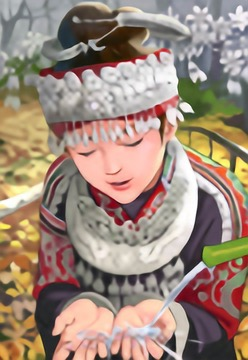
\includegraphics[width=\linewidth]{images/comic_SRResNet-MSE.jpg}
        \caption{SRResNet}
        \label{fig:srgan_srresnet}
    \end{subfigure}
    \begin{subfigure}{.24\linewidth}
        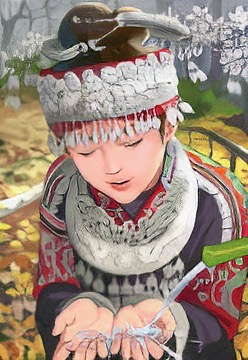
\includegraphics[width=\linewidth]{images/comic_SRGAN-VGG54.jpg}
        \caption{SRGAN}
        \label{fig:srgan_srgan}
    \end{subfigure}

    \caption{Example of single-image super-resolution results that highlight the advantages of a GAN. The original high-resolution image (\ref{fig:srgan_orig}) has been downsampled to make a low-resolution image. The results of bicubic interpolation (\ref{fig:srgan_bicubic}) can be seen in the second image, followed by the results of SRResNet (\ref{fig:srgan_srresnet}), a neural network trained on mean squared error. Lastly, the results of SRGAN can be seen in the final image (\ref{fig:srgan_srgan}). Figure adapted from \textcite{ledig_photo-realistic_2016}.}
    \label{fig:srgan}
\end{figure}

\begin{figure}[t]
    \centering
    \begin{tabular}{ccc}
    Input & Ground Truth & Output \\
    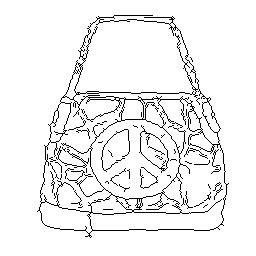
\includegraphics[width=.15\linewidth]{images/handbags_edges_lotsofresults_latex/input_106_AB.jpg} &
    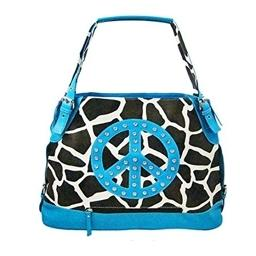
\includegraphics[width=.15\linewidth]{images/handbags_edges_lotsofresults_latex/gt_106_AB.jpg} &
    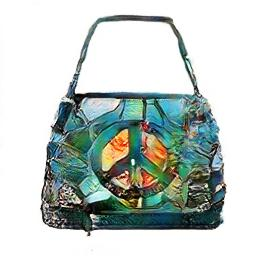
\includegraphics[width=.15\linewidth]{images/handbags_edges_lotsofresults_latex/L1cGAN_106_AB.jpg} \\
    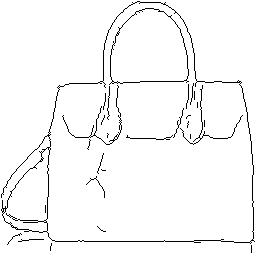
\includegraphics[width=.15\linewidth]{images/handbags_edges_lotsofresults_latex/input_12_AB.jpg} &
    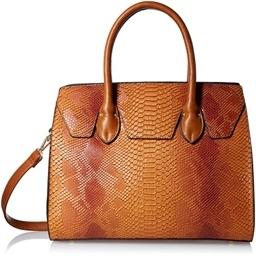
\includegraphics[width=.15\linewidth]{images/handbags_edges_lotsofresults_latex/gt_12_AB.jpg} &
    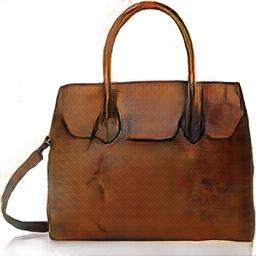
\includegraphics[width=.15\linewidth]{images/handbags_edges_lotsofresults_latex/L1cGAN_12_AB.jpg} \\
    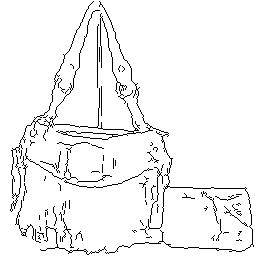
\includegraphics[width=.15\linewidth]{images/handbags_edges_lotsofresults_latex/input_130_AB.jpg} &
    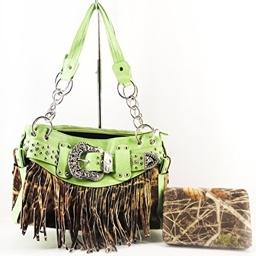
\includegraphics[width=.15\linewidth]{images/handbags_edges_lotsofresults_latex/gt_130_AB.jpg} &
    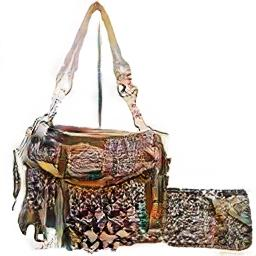
\includegraphics[width=.15\linewidth]{images/handbags_edges_lotsofresults_latex/L1cGAN_130_AB.jpg} \\
    \end{tabular}
    \caption{\textcite{isola_image--image_2016} coined the term image-to-image translation where an input image is transformed into a revisualization of the original input. This figures illustrates how an outline of a purse (leftmost column) is transformed into a colored photorealistic version of it (rightmost column). In the middle we have the ground truth: the real image of the purse. Figure adapted from \textcite{isola_image--image_2016}.}
    \label{fig:pix2pix}
\end{figure}

Having said all of these, the majority of developments with generative models lie in the field of Computer Vision. But that is not to say that we can generate only images. Generative models have been applied with varying degrees of success also in Natural Language Processing - where the scope was to generate high-quality text with sufficient diversity \parencite[e.g.,][]{yu_seqgan_2016, chen_adversarial_2018}. Less explored, but still successful, have been the efforts in generating music \parencite[e.g.,][]{mogren_c-rnn-gan_2016, dong_musegan_2017}. Herein lies the scope of this paper. We evaluated the samples generated by a GAN \parencite{mogren_c-rnn-gan_2016} and LSTM \parencite{oore_this_2018} when trained under a meta-learning algorithm (see Section \ref{sec:hungry}). To reiterate, a full explanation of the purpose of the paper is provided in Section \ref{sec:thesis_goal}.

\section{We always want more}\label{sec:hungry}

DL models usually rely on a procedure called stochastic gradient descent (SGD) which implies computing an output and an error for a given input vector, followed by calculating the input's average gradient and adjusting the network's parameters in a manner that minimizes the error \parencite{lecun_deep_2015}. \textcite{ravi_optimization_2016} argue that the iterative nature of gradient-optimization algorithms does not allow them to perform well under the constraint of a set number of updates over few examples. In particular, when faced with non-convex optimization problems, DL algorithms do not guarantee convergence within a reasonable amount of time. In addition, they also emphasize that for each new problem (e.g., new dataset), the model needs to reinitialize with a new set of random parameters. Ultimately, this hurts the network's ability to converge to a good solution when constrained by a limited number of updates \parencite{ravi_optimization_2016}. Thus they lay out two clear drawbacks of DL models: "data-hunger", and inability to perform separate tasks.

A clear outcome from solving these issues would be that DL models are easier to train (less data) and multifunctional however, this list is not exhaustive. There is also fact that humans have the ability to generalize after one (or few) example(s) of a given object \parencite{vinyals_matching_2016, chen_closer_2018, ravi_optimization_2016} - something which DL models tend to lack. Moreover, there are many fields where the data exhibits a large number of classes, with few examples per class. Bridging the gap between human-type learning and current learning architectures would allow models to properly capture this sort of sparse data \parencite{ravi_optimization_2016, larochelle_few-shot_2017}. This has motivated a series of explorations in the direction of "few-shot" learning (i.e., learning a class from a few examples) or more broadly, into the field of "meta-learning" \parencite[learning to learn in hopes of generalizing to new tasks;][]{chen_closer_2018, vinyals_matching_2016, zhang_metagan_2018}.

In spite of its proposed benefits, developments and experiments with few-shot learning are still scarce \parencite{larochelle_few-shot_2017}. Moreover, evaluations are largely concentrated on image data \parencite[see][]{lake_omniglot_2019, clouatre_figr_2019, vinyals_matching_2016, chen_closer_2018, ravi_optimization_2016}. Having said that, few-shot experiments with generative networks are even less frequent; \textcite{clouatre_figr_2019}, \textcite{dong_musegan_2017} and \textcite{zhang_metagan_2018} being some of the early explorers in this direction.

\section{Composing like a human} \label{sec:thesis_goal}

At the time of writing, generative models and meta-learning are two exciting areas of research in DL which have been successfully combined. However, to the knowledge of the researcher, no such experiments have been conducted in the musical domain. Thus, this paper examined the extent to which generative models can create novel and qualitative samples of music under the constraints posed by few-shot learning. In other words, it sought to evaluate the extent to which generative models can create novel and high-fidelity samples when training data is scarce. To avoid ambiguity, we define novel as new (i.e., not in the training set), and qualitative as consistent with common scales and diverse (combines chord structures with single-note sequences, is not restricted to only a few notes, etc.). This research will evaluate the generated samples of two state-of-the-art generative models (C-RNN-GAN of \cite{mogren_c-rnn-gan_2016} and Performance-RNN of \cite{oore_this_2018}) that have been trained under a meta-learning framework, Reptile \parencite{nichol_first-order_2018}, on a limited number of piano recordings. The performances of these two models were compared to the baseline proposed by \textcite{larochelle_few-shot_2017} and to recorded performances played by expert piano players at the International e-Piano Competition \parencite{university_of_minnesota_international_2019}.

In other words, this study sought to answer the following research questions:

\begin{itemize}
    \item To what extent is the music created by a few-shot generative model comparable to the music of a generative model that is trained on the entire dataset?
    \item To what extent is the music created by a few-shot generative model comparable to real music?
\end{itemize}

The following chapters will discuss more about generative models, meta-learning, and some of the models and algorithms involved in this paper (Chapter \ref{chap:theoretical_framework}), followed by a detailed description of the setup of the experiments (Chapter \ref{chap:methods}), and the results obtained from them (Chapter \ref{chap:results}). Finally, Chapter \ref{chap:discussion} closes with a discussion of the results and limitations of the experimental setup, whereas Chapter \ref{chap:conclusion} draws some conclusions that answer the above research questions.

\chapter{Related Work}\label{chap:theoretical_framework}

This chapter takes a deep-dive into the fields of meta-learning and generative networks in order to highlight their current state of affairs. This will lay the groundwork for the experiments detailed in Chapter \ref{chap:methods}. Section \ref{sec:rnn} will present the principal network architecture of this paper, the recurrent neural network, and argument for its use as the foundation of a generative network. Section \ref{sec:generative} will introduce Generative Adversarial Networks, a training method build specifically for the task, whereas Section \ref{sec:learn2learn} will formally introduce meta-learning, several approaches to it, and finally narrow down to current state-of-the-art algorithms. 

\section{Recurrent Neural Networks} \label{sec:rnn}

In a standard ANN, the data traverses the network through the input layer, to the hidden layer, and finally reaches the output layer; setup which is generally known as a feedforward neural network \parencite[Figure \ref{fig:feedforward_net};][]{graves_supervised_2012}. Broadly, this type of network is defined by the fact that its connections do not form cycles. If however we relax this condition, we arrive at a recurrent neural network \parencite[Figure \ref{fig:rnn_folded};][]{rumelhart_learning_1986}: a family of neural networks specifically designed for processing sequential data \parencite{goodfellow_deep_2016}. It is possible to use a feedforward architecture, specifically a one-dimensional Convolutional Neural Network, with sequential data, where the convolution would be the basis for building a time-delay neural network. Unfortunately, the output of such a network would be a function of a small number of neighbouring data points \parencite[say, the last three notes;][]{goodfellow_deep_2016} whereas in the contex of music, knowledge of the notes played from the begining of the song is needed. As such, RNNs seem to be a more compelling alternative for this task.

The information passes through the RNN in a similar manner to the feedforward network except that the activations which arrive at the hidden layer are from the current external input and prior hidden activations from the previous timestep \parencite{graves_supervised_2012}. Moreover, recurrent networks also benefit from the fact that parameters (weights) are shared across different parts of a model. This allows extending and applying the model to data points of different lengths and generalizing across all of them \parencite{goodfellow_deep_2016}. In contrast, a feedforward network would require separate parameters for each input feature, at each position. Thus, a formal definition of the network's forward pass would be
\begin{equation}
    h^t = f(h^{t-1}; x^t; \theta) \label{eq:rnn_hidden}
\end{equation}
where $h^t$ is the state of the hidden layer at time $t$, $x^t$ is the input at time $t$, and $\theta$ the model parameters.

The backward pass in a RNN is similar to that of a feedforward network: given the partial derivatives of a differentiable loss function $\mathcal{L}$ we calculate the derivatives with respect to the network's weights \parencite{graves_supervised_2012}. In this setting, a popular algorithm is called backpropagation through time \parencite[BPTT;][]{werbos_backpropagation_1990} which consists of repeated applications of the chain rule. The difference between standard backpropagation and BPTT is that the loss function depends on the activation of the hidden layer through its influence on the output layer as well as its influence on the hidden layer a the next timestep \parencite{graves_supervised_2012}.

Equation \ref{eq:rnn_hidden} can be drawn as in Figure \ref{fig:rnn_folded}: input sequences $x$ are mapped to a hidden layer $h$ and an output $y$, with the state of the hidden layer at time $t$ feeding back into itself with a time delay of $1$. In other words, the state of $h_t$ will influence the decision of the recurrent layer at time $t+1$. Another way to illustrate this is to unfold the computational graph such that each component of the network is represented by different variables per step, as in Figure \ref{fig:rnn_unfolded}.

The reason why these notions have been introduced is to be able to bring up the following point. As good as standard RNNs are - in theory - at accessing contextual information when mapping input sequences to output sequences, the range of contexts that can be accessed in a standard RNN architecture is in practice quite limited \parencite{graves_supervised_2012}. \textcite{hochreiter_long_1997} outlines two problems caused by BPTT: the error signals flowing bacwards in time tend to either (1) blow up or (2) vanish. As such, the Long Short-Term Memory network has been proposed, a recurrent architecture designed to overcome these issues \parencite{hochreiter_long_1997}.

\begin{figure}[t]
    \centering
    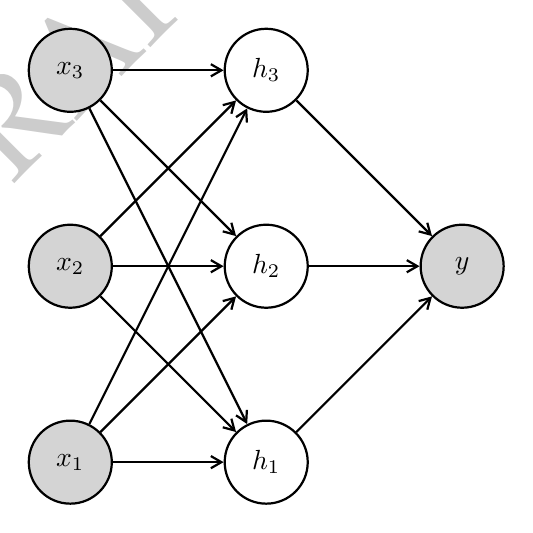
\begin{tikzpicture}
        \node[io] (x1) {$x_1$};
        \node[io, above=4em of x1] (x2) {$x_2$};
        \node[io, above=4em of x2] (x3) {$x_3$};

        \node[neuron, right= of x1] (h1) {$h_1$};
        \node[neuron, above=4em of h1] (h2) {$h_2$};
        \node[neuron, above=4em of h2] (h3) {$h_3$};

        \node[io, right= of h2] (y) {$y$};

        \foreach \x in {1, 2, 3}
            \foreach \h in {1, 2, 3}
                \draw[conn] (x\x) -- (h\h);

        \foreach \h in {1, 2, 3}
            \draw[conn] (h\h) -- (y);
    \end{tikzpicture}
    \caption{Example of a feedforward neural network with three nodes in the input layer ($x_1$, $x_2$, $x_3$), three nodes in the hidden layer ($h_1$, $h_2$, $h_3$), and an output layer a single node ($y$).}
    \label{fig:feedforward_net}
\end{figure}

\begin{figure}[t]
    \centering
    \begin{subfigure}{.24\linewidth}
        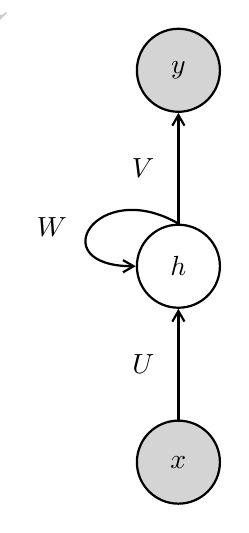
\begin{tikzpicture}
            [align=center]
            % Draw recurrent network
            \node[neuron] (h) {$h$};
            \node[io, below=4em of h] (x) {$x$};
            \node[io, above=4em of h] (y) {$y$};

            \draw[conn] (h) -- node [left=0.5em, midway, align=center] {$V$} (y);
            \draw[conn] (x) -- node [left=0.5em, midway, align=center] {$U$} (h);
            \draw[conn] (h.north) to [out=150, in=180, loop, looseness=4] node[left=0.5em, midway, align=center] {$W$} (h.west);

        \end{tikzpicture}
        \caption{Folded}
        \label{fig:rnn_folded}
    \end{subfigure}
    \begin{subfigure}{.74\linewidth}
        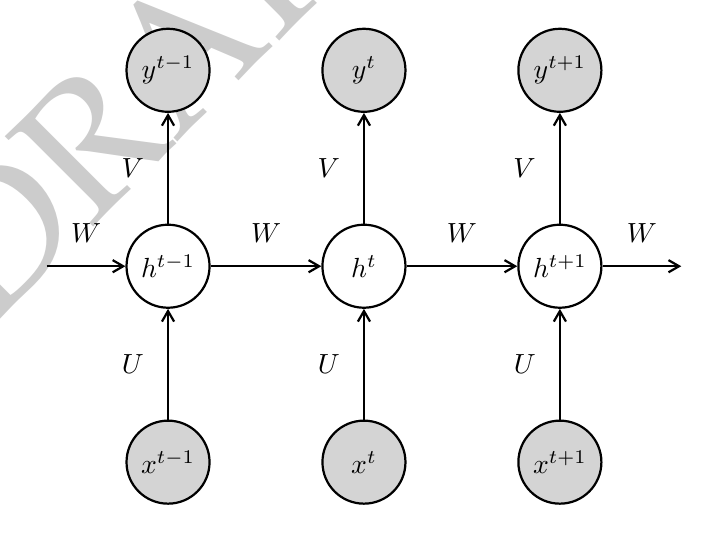
\begin{tikzpicture}
            [align=center]
            % Draw middle unfold
            \node[neuron] (ht) {$h^t$};
            \node[io, below=4em of ht] (xt) {$x^t$};
            \node[io, above=4em of ht] (yt) {$y^t$};

            \draw[conn] (ht) -- node [left=0.5em, midway, align=center] {$V$} (yt);
            \draw[conn] (xt) -- node [left=0.5em, midway, align=center] {$U$} (ht);

            % Draw left unfold
            \node[neuron, left = of ht] (ht-1) {$h^{t-1}$};
            \node[io, below=4em of ht-1] (xt-1) {$x^{t-1}$};
            \node[io, above=4em of ht-1] (yt-1) {$y^{t-1}$};

            \node[left= of ht-1] (nullLeft) {};

            \draw[conn] (ht-1) -- node [left=0.5em, midway, align=center] {$V$} (yt-1);
            \draw[conn] (xt-1) -- node [left=0.5em, midway, align=center] {$U$} (ht-1);

            \draw[conn] (ht-1) -- node [above=0.5em, midway, align=center] {$W$} (ht);
            \draw[conn] (nullLeft) -- node [above=0.5em, midway, align=center] {$W$} (ht-1);
            % Draw right unfold
            \node[neuron, right= of ht] (ht+1) {$h^{t+1}$};
            \node[io, below=4em of ht+1] (xt+1) {$x^{t+1}$};
            \node[io, above=4em of ht+1] (yt+1) {$y^{t+1}$};

            \node[right= of ht+1] (nullRight) {};

            \draw[conn] (ht+1) -- node [left=0.5em, midway, align=center] {$V$} (yt+1);
            \draw[conn] (xt+1) -- node [left=0.5em, midway, align=center] {$U$} (ht+1);

            \draw[conn] (ht) -- node [above=0.5em, midway, align=center] {$W$} (ht+1);
            \draw[conn] (ht+1) -- node [above=0.5em, midway, align=center] {$W$} (nullRight);

        \end{tikzpicture}
        \caption{Unfolded}
        \label{fig:rnn_unfolded}
    \end{subfigure}
    \caption{A typical view of an RNN (left) and an unfolded view of the same network (right). In both sub-figures each node is a layer of network units however, in the second representation these are shown for each timestep. The weighted connections from the input layer to the hidden one is labelled $U$, those from the hidden layer feeding back to itself are $W$, and those from the hidden layer to the output layer are labelled as $V$. Note that these weights are reused at each timestep. Bias has been omitted in this representation. Figure adapted from \textcite{graves_supervised_2012}}
\end{figure}

The LSTM is made of a network of recurrently connected subnetworks known as memory blocks, each with one or more self-connected memory cells and three multiplicative units: the input gate, the output gate, and the forget gate \parencite{hochreiter_long_1997}. The three gates act as analogies for the read, write, reset computer operations and allow the memory cells to store and access information over long periods of time \parencite{graves_supervised_2012}. See Figure \ref{fig:lstm} for an illustration of a LSTM memory block with a single cell.

Aside from being successful at a variety of classification tasks \parencite[e.g.,][]{graves_framewise_2005}, this architecture has been successfully applied to generating new data points \parencite[such as creating sequences of text;][]{graves_generating_2013}. In the context of generating musical performances, experiments with this neural architecture go as far as \textcite{eck_first_2002} however, a more noteworthy implementation is Performance-RNN \parencite{oore_this_2018}; a three layer LSTM network with 512 cells each designed to generate classical compositions whilst maintaining the playing style of expert pianists. Considering how successful it was, this model will be re-implemented in this paper's experiments (see Chapter \ref{chap:methods}).

\begin{figure}[t]
    \centering
    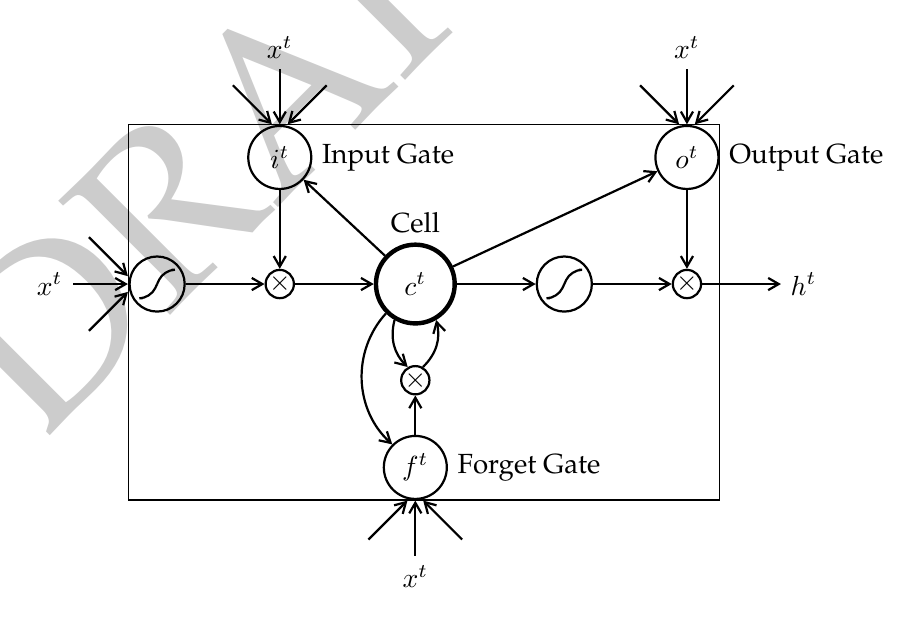
\begin{tikzpicture}
        \node[ct, label={Cell}] (ct) {$c^t$};
        \node[filter, right=of ct] (int1) {};
        \node[prod, right=of int1] (x1) {$\times$}; 
        \node[right=of x1] (ht) {$h^t$};
        \node[prod, left=of ct] (x2) {$\times$}; 
        \node[filter, left=of x2] (int2) {};
        \node[prod, below=5mm of ct] (x3) {$\times$}; 
        \node[ft, below=5mm of x3, label={right:Forget Gate}] (ft) {$f^t$};
        \node[ft, above=of x2, label={right:Input Gate}] (it) {$i^t$};
        \node[ft, above=of x1, label={right:Output Gate}] (ot) {$o^t$};

        \foreach \i/\j in {int2/x2, x2/ct, ct/int1, int1/x1,
                        x1/ht, it/x2, ct/it, ct/ot, ot/x1, ft/x3}
                            \draw[->, conn] (\i)--(\j);

                            \draw[->, conn] (ct) to[bend right=45] (ft);

                            \draw[->, conn] (ct) to[bend right=30] (x3);
                            \draw[->, conn] (x3) to[bend right=30] (ct);

                            \node[fit=(int2) (it) (ot) (ft), draw, inner sep=0pt] (fit) {};

                            \draw[<-, connl] (fit.west|-int2) coordinate (aux)--++(180:7mm) node[left]{$x^t$};
                            \draw[<-, connl] ([yshift=1mm]aux)--++(135:7mm);
                            \draw[<-, connl] ([yshift=-1mm]aux)--++(-135:7mm);
                                         
                            \draw[<-, connl] (fit.north-|it) coordinate (aux)--++(90:7mm) node[above]{$x^t$};
                            \draw[<-, connl] ([xshift=1mm]aux)--++(45:7mm);
                            \draw[<-, connl] ([xshift=-1mm]aux)--++(135:7mm);
                                          
                            \draw[<-, connl] (fit.north-|ot) coordinate (aux)--++(90:7mm) node[above]{$x^t$};
                            \draw[<-, connl] ([xshift=1mm]aux)--++(45:7mm);
                            \draw[<-, connl] ([xshift=-1mm]aux)--++(135:7mm);
                                          
                            \draw[<-, connl] (fit.south-|ft) coordinate (aux)--++(-90:7mm) node[below]{$x^t$};
                            \draw[<-, connl] ([xshift=1mm]aux)--++(-45:7mm);
                            \draw[<-, connl] ([xshift=-1mm]aux)--++(-135:7mm);
    \end{tikzpicture}
    \caption{LSTM memory block with one cell. Here the gates are nonlinear summation units that collect activations from the inside and outside of the memory block and control the activation of the cell $c^t$ via multiplications. The input and output gates ($i^t$, $o^t$) multiply the block's input and output activations respectively, while the forget gate ($f^t$) multiplies the previous hidden state. The input and output activation are typically tanh or sigmoid. The only outputs ($h^t$) from the block come from the output gate multiplication. Figure adapted from \textcite{graves_supervised_2012}}
    \label{fig:lstm}
\end{figure}

\section{Generative Adversarial Networks} \label{sec:generative}

Nowadays, the most popular form of generating data is through the use of a Generative Adversarial Network \parencite[GAN;][]{goodfellow_generative_2014}. The training procedure is set up as a game between two networks: a generator and a discriminator. The purpose of the former is to create samples that come from the same distribution as the training data, whereas the latter aims to determine which samples are real or fake \parencite{goodfellow_nips_2016}.

To make the generator's data distribution $p_g$ imitate that of the real data $p_{\text{data}}$, we need to define a prior on input noise variables $p_{z}(z)$ and then represent a mapping to the data space $G(z; \theta_g)$ where $G$ is a differentiable function represented by a network with parameters $\theta_g$. The discriminator is another network with a mapping function $D(x; \theta_d)$ that outputs a single scalar where $D(x)$ is the probability that $x$ came from the real data distribution rather than that of the generator \parencite{goodfellow_nips_2016}. We train $D$ to maximize the probability of correctly assigning a label to the training data and samples from $G$ ("real" and "fake"), while simultaneously training $G$ to minimize the dissimilarity between the two data distributions, without actually looking at $p_{\text{data}}$. In other words, $G$ must minimize $\log (1- D(G(z)))$ \parencite{goodfellow_generative_2014}.

In other words, both models play a minimax game with a value function $V(G, D)$:
\begin{equation}
    \min_G \max_D V(D, G) = \mathbb{E}_{x ~ p_{\text{data}}} [ \log D(x) ] + \mathbb{E}_{z ~ p_z (z)} [ \log (1-D(G(z))) ]
\end{equation}
where the solution is for $G$ to recover the training data distribution and $D$ to have a classification accuracy of 50\% \parencite{goodfellow_generative_2014}.

Although new, GANs are a significant conceptual and technical innovation \parencite{briot_deep_2017} which can be seen in them revitalizing interest in generative models. As mentioned before, they have been proven successful at image super-resolution \parencite{ledig_photo-realistic_2016}, image-to-image translation \parencite{isola_image--image_2016}, or style-based image generation \parencite{karras_style-based_2018}. Having said these, \textcite{mogren_c-rnn-gan_2016} has shown that GANs do not belong only to the field of Computer Vision by re-purposing this architecture to generate music. The model in question, C-RNN-GAN, features a completely unidirectional LSTM network with two layers, 350 units each as generator and a unidirectional LSTM network with a similar structure as discriminator.

\section{Learning to learn} \label{sec:learn2learn}

The rationale for investing time and energy into meta-learning is that we cannot capture the essence of learning simply by relying on a small number of algorithms, but rather a bunch of context-dependent learning strategies that would enable us to properly capture domain specific information \parencite{schmidhuber_evolutionary_1987}. Given the complexities of each learning strategy, \textcite{schmidhuber_evolutionary_1987} argues that an obvious way to tackle this initiative is to give a system the ability to learn how to learn. A simplistic way to do this would be to train a system on different tasks (e.g, image classification, text classification, etc.). However, this approach entails training on a dataset that is much larger that what current hardware can withstand. Furthermore, this approach would stray away from the idea of building general-purpose A.I. architectures as generalizing over a task would require more data points that what a human would need. To be more concrete, a human is able to generalize a task/object after encountering one (or few) example(s) \parencite{ravi_optimization_2016, chen_closer_2018}. Therefore, besides having to perform on a variety of tasks, a systems would need to excel at that using sparse amounts of data.

Although ideas of meta-learning can go as far as Schmidhuber's thesis in 1987, it seems that training a network using a handful of examples did not get much traction until \textcite{lake_human-level_2015} successfully designed a probabilistic learning framework capable of generalizing and learning a large number of concepts from a single class example (i.e., one-shot learning). For clarity, such a problem is typically defined as a $n$-shot $k$-way problem, where $n$ stands for the number of examples per class, and $k$ is the number of classes to be used in the training process.

Initially, it was thought that such a framework would not work in the context of an ANN since the iterative nature of gradient-based optimization algorithms do work well in the context of a set number of updates \parencite{ravi_optimization_2016} - and even more so when there are only a few examples to work with. Having said that, \textcite{rezende_one-shot_2016} were among the first to provide a solution to the one-shot problem in the context of a neural network by implementing Bayesian reasoning into a deep network embedded within hierarchical latent variable models. Since that, numerous efforts were made to develop an algorithm that enables an ANN to perform with a constrained number of class examples. Probably the most popular algorithm at the time of writing is the Model-Agnostic Meta-Learning (MAML) algorithm \parencite{finn_model-agnostic_2017}. One of MAML's core mechanics is the parameter update by calculating second-order derivatives. This procedure however implies a substantial computational penalty, which the authors did note. Therefore, they developed a first-order variant of MAML (FOMAML) which is able to perform similarly, if only slightly worse \parencite{finn_model-agnostic_2017}.

This however, seemed to be the initial thought, until \textcite{nichol_first-order_2018} showed that FOMAML tends to be somewhat unstable and very sensitive to even the smallest changes in hyper-parameters. Therefore, they developed Reptile, a first-order meta-learning algorithm that rivals both MAML and FOMAML \parencite{nichol_first-order_2018}. Just like MAML, it counteracts the shortcomings of gradient-optimization algorithms by learning the model's initial parameters in order to maximize performance on novel tasks, it allows for any type of network to be used, and does not place any restrictions on the type of loss function that can be used \parencite{nichol_first-order_2018}. The difference between the two however, lies in the way the parameters are updated. 

\IncMargin{1em}
\begin{algorithm}
Initialize $\theta$, the vector of initial parameters

\For{iteration = $1, 2, \dots$}{
    Sample task $\tau$, corresponding to loss $L_{\tau}$ on weight vectors $\tilde \theta$

    Compute $\tilde \theta = U_{\tau}^{k} (\theta)$, denoting $k$ steps of SGD or Adam

    Update $\theta \leftarrow \theta + \epsilon (\tilde{\theta} - \theta)$
}

\caption{Reptile (serial version)}
\label{alg:reptile}
\end{algorithm}
\DecMargin{1em}

In essence, the way Reptile works (see Algorithm \ref{alg:reptile}) is as follows. A model with parameters $\theta$ is initialized, and a meta-loop (or meta-epochs) of $i$ iterations starts. Within it, a task $\tau$ (e.g, image classification, text classification, etc.) is sampled, along with its corresponding loss function $L_{\tau}$ (for clarity we assume that each type of task uses a different loss function). Then we compute the updated parameters $\tilde \theta$ in an inner-loop with $k$ iterations on task $\tau$ (or in other words, once we sampled our task $\tau$, we train our model $k$ times on it using the $\theta$ as parameters so we can get $\tilde \theta$). Finally, we update out initial parameters $\theta$ using this formula: $\theta \leftarrow \theta + \epsilon (\tilde{\theta} - \theta)$. Then the algorithm continues to the next iteration of the meta-loop carrying over our updated parameters $\theta$.

The explanation above is fairly verbose however, the algorithm itself is fairly simplistic but achieves similar performances to FOMAML \parencite{nichol_first-order_2018}. This forms a compelling reason to use Reptile as the few-shot learning method of choice for this paper.

\chapter{Methods}\label{chap:methods}

To reiterate from Section \ref{sec:thesis_goal}, the purpose of this paper is to establish (1) the extent to which the music generated under a few-shot learning algorithm is comparable to that of a model trained on the entire dataset, and (2) the extent to which the music from such a model is comparable to that of real musical performances. For these purposes, Performance-RNN and C-RNN-GAN were adapted to the Reptile training procedure (Algorithm \ref{alg:reptile}) and evaluated against the performances generated by the baseline proposed in \textcite{larochelle_few-shot_2017} - a single layer LSTM with 256 units - and actual musical performances from the dataset (Section \ref{sec:dataset}). For an in-depth explanation on the steps required to develop a model that is able to generate new data points refer to Section \ref{sec:how_to_gen} and to Section \ref{sec:reptile_train} for details on the training procedure. The evaluation of the models' performances will be based on the number of statistically different bins \parencite[NDB;][]{richardson_gans_2018} and several domain specific measurements adapted from \textcite{mogren_c-rnn-gan_2016}: polyphony, scale consistency, repetitions, tone span. Refer to Section \ref{sec:evaluation} for more details on these metrics.

\section{Dataset} \label{sec:dataset}

The dataset for this research will be similar to that of \parencite{oore_this_2018} namely, the MAESTRO Dataset \parencite{hawthorne_enabling_2018}. It consists of recorded MIDI data collected from each installment of the International Piano-e-Competition. All performances were done by piano experts on a Yamaha Disklavier, instrument which integrates a highly precise MIDI capture and playback system. The claim is that the recorded MIDI events are of sufficient fidelity to allow judges to remotely listen to the contestant's performance (also on a Disklavier).

The dataset contains MIDI recordings from nine years of the International Piano-e-Competition. This amounts to 1,184 piano performances, approximately 430 compositions, 6.18 million notes played, and approximately 172 hours of playback. There is also a recommended train/validation/test split (954, 105, 125 songs respectively) created on the following criteria \parencite{hawthorne_enabling_2018}:

\begin{itemize}
    \item No composition should appear in more than one split
    \item Training set is approx 80\% of the dataset (in time), and the remaining is split equally on between the validation and test sets. Where possible, these proportions are true also within each composer.
    \item Popular compositions are in the training set
    \item The validation and test splits should maintain a variety of compositions
\end{itemize}

Moreover, each performance comes with additional metadata such as, the name of the composer, the title of the performance, the suggested train, validation, test splits, year of the performance, name of the file, and duration in seconds of the performance. Having said that, the dataset lacks clearly defined classes. The canonical composer could be used as a substitute however, the author strongly believes that there is a better way to categorize music: by genre.

Broadly speaking, Western classical music can be segregated into a number of genres based on the year of the composition and style of the piece. For this we can use the Concise Oxford Dictionary of Music \parencite{kennedy_concise_2007} which indicates to the following classical genres: baroque (1600 - 1750), classical (1750 - 1820), romanticism (1780 - 1910), modernism (1890 - 1930), and impressionism (circa 1890 - 1925). Granted, there are far more genres, but these are the ones that are covered by the dataset. As such, given the definitions of \textcite{kennedy_concise_2007} on said genres and artists, each individual piece from our dataset was manually assigned a genre. Concretely, the style of music was firstly determined by the period in which the composer has lived (in baroque, classical, etc.) or - if the genres would overlap (i.e., modernism, and impressionism) - the composer's primary style of music would be chosen according to the definition of the composer given by \textcite{kennedy_concise_2007}. Said labelling can be found in Appendix \ref{appendix:labelling}.

\section{Data Processing} \label{sec:data_proc}

\begin{figure}[t]
    \centering
    \begin{verbatim}
<note_on note=69 velocity=73 time=33>
<note_on note=71 velocity=78 time=15>
<control_change control=64 value=83 time=27>
<note_off note=69 velocity=0 time=6>
<note_off note=71 velocity=0 time=3>
    \end{verbatim}
    \caption{Example of MIDI messages in the dataset, as printed by the Python library Mido \parencite{bjorndalen_mido_2018}. At 33 ticks since the last event, the player pressed an A4 (note 69), followed by a B4 (note 71), 15 ticks later. Next, the pedal (Control Change message with a value of 64) is pressed 27 ticks later, and the keys are released 6 and 3 tick later.}
    \label{fig:midi_examples}
\end{figure}

The dataset consists of MIDI files which would require some processing in order to be ready for a LSTM network. Here, the approach of \textcite{oore_this_2018} was adopted where MIDI midi messages are transformed into a sequence of one-hot encoded events. More specifically, MIDI excerpts are represented as a sequence of events from a vocabulary of 416 different events - similar to \textcite{oore_this_2018}, but with three extra events in the vocabulary:
\begin{itemize}
    \item 128 Note-On events: starts a new note (one for each of the 128 MIDI pitches)
    \item 128 Note-Off events: releases a note (one for each of the 128 MIDI pitches)
    \item 126 Time-Shift events: moves the time step forward somewhere between 0 ms and 1 second, in increments of 8 ms
    \item 32 Velocity events: changes the velocity for each subsequent note, until the next velocity event
    \item 2 Pedal events: triggers or releases the pedal
\end{itemize}

A glance over the MIDI documentation \parencite{midi_association_official_2019} shows how complex and granular the standard is. However, we do not need to implement all of the messages into our model in order to make it work. We only need three: \texttt{note\_on}, \texttt{note\_off}, \texttt{pedal\_on/off}. Figure \ref{fig:midi_examples} show an example of how the midi messages look like. It should be noted that in this figure, the time is represented in ticks, MIDI's smallest unit of time, who's value is usually a third of a beat \parencite{midi_association_official_2019}.

As it can be seen in Figure \ref{fig:midi_examples}, each message contains multiple pieces of information such as the message type, the note/value of the message, the delta time (time elapsed since last message and the current message, measured in ticks), and velocity (if applicable). To one-hot encode this stream of messages, it is necessary to separate it so it contains only one type of information per entry. Thus, the sequence can be further broken down such that the first message that the system encounters is the delta time, followed by the velocity, and the note/pedal event (and their respective values). An example of how the MIDI sequences are broken down into singular pieces of information can be found in Figure \ref{fig:representation_midi}.

\begin{figure}[t]
    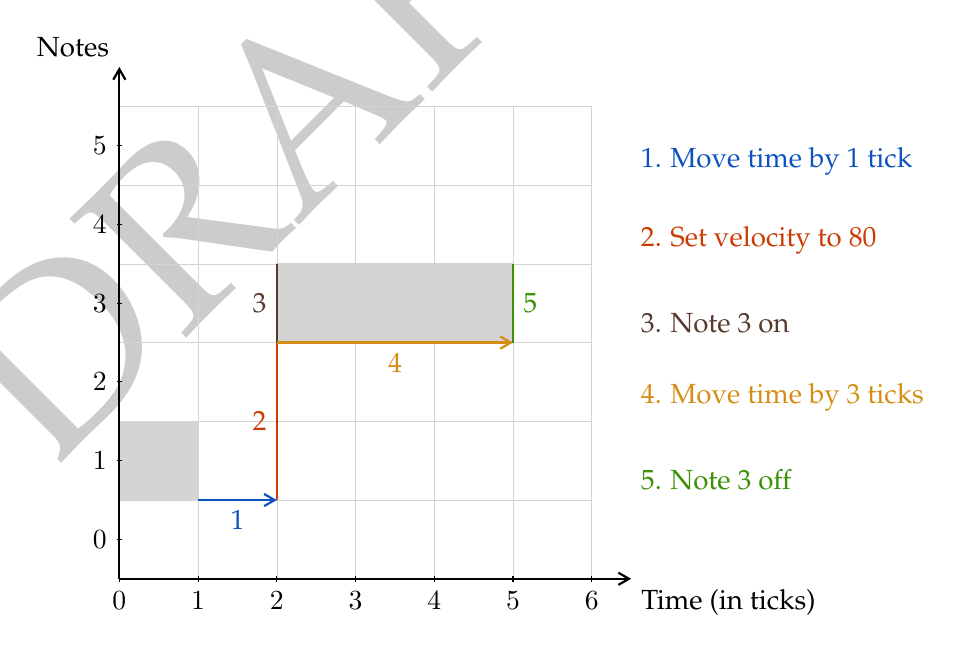
\begin{tikzpicture}
        \draw[step=1cm,base01,very thin] (0,0) grid (6,6);
        \filldraw[fill=base01, draw=base01] (0,1) rectangle (1,2);
        \filldraw[fill=base01, draw=base01] (2, 3) rectangle (5, 4);
        \draw (6.5, 5) node[anchor=south west, color=base09] {1. Move time by 1 tick};
        \draw (6.5, 4) node[anchor=south west, color=base0A] {2. Set velocity to 80};
        \draw (6.5, 3) node[anchor=south west, color=base0B] {3. Note 3 on};
        \draw (6.5, 2) node[anchor=south west, color=base0C] {4. Move time by 3 ticks};
        \draw (6.5, 1) node[anchor=south west, color=base0D] {5. Note 3 off};

        \draw[ -{Straight Barb[angle=60:2pt 3]}, color=base09, thick] (1, 1) -- (2, 1) node[anchor=north, midway] {1};
        \draw[color=base0A, thick] (2, 1) -- (2, 3) node[anchor=east, midway] {2};
        \draw[color=base0B, thick] (2, 3) -> (2, 4) node[anchor=east, midway] {3};
        \draw[ -{Straight Barb[angle=60:2pt 3]}, color=base0C, thick] (2, 3) -- (5, 3) node[anchor=north, midway] {4};
        \draw[color=base0D, thick] (5, 3) -- (5, 4) node[anchor=west, midway] {5};

        \draw[thick,-{Straight Barb[angle=60:2pt 3]}] (0,0) -- (6.5,0) node[anchor=north west] {Time (in ticks)};
        \draw[thick,-{Straight Barb[angle=60:2pt 3]}] (0,0) -- (0,6.5) node[anchor=south east] {Notes};
        \foreach \x in {0,1,2,3,4,5,6}
           \draw (\x cm,1pt) -- (\x cm,-1pt) node[anchor=north] {$\x$};
        \foreach \y in {0,1,2,3,4,5}
            \draw (1pt,\y.5 cm) -- (-1pt,\y.5 cm) node[anchor=east] {$\y$};
    \end{tikzpicture}
    \caption{Example of how the data is represented. The progression illustrates how a piano roll of MIDI data is converted into a sequence of commands (right hand side) that belong to our events vocabulary. Figure adapted from \textcite{oore_this_2018}.} 
    \label{fig:representation_midi}
\end{figure}

Having said these, it should be mentioned that the one-hot representation of MIDI messages has undergone some fine quantization, again, in a similar fashion to \textcite{oore_this_2018}. The delta times have been modified to correspond to a change of multiples of 8 ms (i.e., 0 ms, 8 ms, 16 ms, etc.) and the velocities have been partitioned into 32 steps as opposed to MIDI's 128. With regards to the time movements, \textcite{friberg_overview_2006} note that a noticeable difference in temporally displacing a single tone in a sequence takes place from 10 ms and above. When in comes to the note velocities, it should be pointed to the reader that classical music features eight levels of common dynamic marking (from $ppp$ to $fff$) which is why \textcite{oore_this_2018} note that 32 steps are more than enough.

\section{You're a musician Schmidhuber} \label{sec:how_to_gen}

Knowing what we know about RNNs and LSTMs from Section \ref{sec:rnn} one can devise a method where the network can generate a sequence of events. All that is needed is to present the system with an event to kickstart the generative process. Namely, an input $x^t$ of size 1 is given to the network to output the next likely event $x^{t+1}$, which in turn is fed back to generate $x^{t+2}$. This process is repeated until we have a sequence of events of a desired length.

An alternative to this would be to define a noise vector $z^t$ of an arbitrary size (e.g., 100), and a random input $x^t$ selected from our events vocabulary. The noise vector is passed through a linear layer that output a tensor that would serve as the network's hidden state $h^{t}$ at time $t$. It is then that $x^t$ and $h^{t}$ are fed into the LSTM layer to generate $x^{t+1}$ and $h^{t+1}$. The reason for pre-defining the hidden state for the first input is to increase the number of possible outcomes coming from the network.

To be more precise, if we were to present the network with only $x^t$ then the network would mark the input sequence as the beginning of the song. With that information, it is possible that the network would affix itself to following a specific pattern. For instance, if the first input would be a C\#, the network could learn to always output E as the next note. Using a random hidden state is a measure that was included to ensure some diversity in the process of generating samples (granted, it should be admitted the possibility of this scenario being unlikely, and that the regular method described above would still work just as good).

Having said this, diversity is not the only reason for including a noise vector $z$ into the training process. The reader might recall that this is part of the generation process in the framework of a GAN respectively, how the generator $G$ would create samples. Hence, all three models implemented in this paper feature the architecture of a GAN generator.

In terms of generating the next event, \textcite{oore_this_2018} have defined a parameter $\tau$ called temperature \parencite{google_magenta_performance_2017}. It is a value which uses the model's predicted events distribution to control the randomness of the output samples. In other words, let $\phi$ be the output of a LSTM network (for clarity, we ignore the hidden state $h$). Then, the next sequence $x^{t+1}$ is defined as 
\begin{equation}
    x^{t+1} = X(\omega)
\end{equation}
where
\begin{equation}
    X = \text{softmax}(\phi / \tau).
\end{equation}
$X$ is the predicted event distribution of the network's output divided by our temperature $\tau$. Thus, $x^{t+1}$ is actually a random sample from our defined categorical distribution $X$.

\section{How to train a Reptile} \label{sec:reptile_train}

With the generative process outlined in the previous section, training the generative networks outlined in this papers is somewhat straightforward. A batch of songs is sampled from the training set, the model generates as many songs as there are in the batch, and then compute the loss between the network's output and the real samples. This statement is essentially true for the baseline and PerformanceRNN (in spite of the Reptile training procedure, inner-loop training is similar to the standard procedure). In contrast, the GAN model requires training two models simultaneously, where the generator's loss function is based on whether the discriminator is fooled by the fake samples (i.e., classifies them as real), and the discriminator's loss is based on whether it can distinguish between real and fake samples (it should be mentioned that both models would use binary cross-entropy as their loss function). However, there are still several items that we haven't touched upon.

Firstly, all three networks have been trained with teacher forcing, a procedure in which during training the model receives the ground truth $y^t$ as input at time $t+1$. Adopting this measure allows the model to create hidden-to-hidden connections and capture the necessary information from the history of input sequences \parencite{goodfellow_deep_2016}.

Secondly, \textcite{goodfellow_generative_2014} mention a couple issues that can arise when training a GAN. One is synchronizing the generator with the discriminator (it's possible that one of the models gets too strong, leaving the other unable to catch up), and the generator collapsing too many values of $z$ to the same value of $x$ (which would ultimately hurt the generator's diversity; this issue is known in the literature as mode collapse).

A solution to the issue of synchronicity would be to freeze the training of one of the models when the loss is below a predefined threshold \parencite{mogren_c-rnn-gan_2016}. In this paper, we stop training one of the models when its training loss is less than half the loss of the other's.

To combat mode collapse, \textcite{salimans_improved_2016} propose a technique called feature matching, where we change the objective of the generator to generate real data that matches the statistics of the real data. Since in the setting of a GAN showing the real data would be considered "cheating", we use the features of an intermediate layer of the discriminator. Specifically, we train the generator to match the expected value of those features \parencite{salimans_improved_2016}. Denoting $f(x)$ as the activations on an intermediate layer in the discriminator, the new objective for the generator becomes
\begin{equation}
    \|\mathbb{E}_{x~p_{data}} f(x) - \mathbb{E}_{z~p_z (z)} f(G(z))\|_2^2
\end{equation}
which is commonly known as the squared error. However, to make the re-implementation of C-RNN-GAN true to the original, Mean Square Error (MSE) was used as the loss function when using feature matching.

It should be noted that now, the loss functions of both the generator and discriminator differ in scale, meaning that we can no longer compare them to freeze training of either models: the generator uses MSE, whereas the discriminator use binary cross-entropy. A workaround to this is to calculate the both losses, but use MSE for backpropagation and optimization, whilst binary cross-entropy is used to compare our models.

Moving forward, there is an aspect pertaining to the Reptile training framework which needs to be addressed: the training data. Normally, Reptile assumes that the training takes place in the $n$-shot $k$-way setting, meaning that our model is trained with $k$ classes and $n$ samples per class. Given that we have 954 samples in the training set, we adopted the same training procedure as \textcite{nichol_first-order_2018} and \textcite{clouatre_figr_2019}. Respectively, at each meta-loop we sample from our split $n$ examples for each $k$ class. For this paper, our $n=1$ and $k=5$ corresponding to a 5-way 1-shot experiment.

Another aspect that needs addressing is the number of epochs. All models were trained for 250 epochs each however, when looking at the way training is handled in Reptile (see Algorithm \ref{alg:reptile}), this statement is inconclusive. Because the algorithm presents us with a meta-loop and an inner-loop, epochs is defined in this setting as the number of times parameters $\theta$ have been updated. Thus, the number of steps we have taken to compute $\tilde \theta$ is ignored. If there is skepticism about the fact that the Reptile models are trained much more than the baseline leading to better performances, the reader should be reminded by the fact that the latter is presented with 954 songs per epoch, whereas the former are trained with five.

With these in mind, it should be mentioned that neither of the three models was presented with a full song during training, but rather with each song split into fixed-size chunks. This decision was made to better accommodate the memory limits of the hardware (an Nvidia T4 GPU). A full explanation of the limitations is found in Appendix \ref{appendix:memory}. It suffices to say that our dataset won't fit in memory. As such, each song was split into chunks of 200 events (i.e., window size of 200), starting from the beginning and moving towards the end of the song at a rate of 50 events per chunk (i.e, stride size of 50). Thus, a song of, say, 800 events would be transformed into 13 chunks, which leads us to the topic of batch size.

At training, the Reptile models were presented with batches of 64 chunks, whereas the baseline was presented with batches of 2048 chunks. The rationale for the latter is that training of the baseline under a regimen of 64 batches would take approximately 250 hours until completion.

Finally, another aspect that needs addressing is the learning rate. The baseline and Reptile inner-loop training was conducted with an $\alpha = 0.001$, value borrowed from \textcite{oore_this_2018}. Since Reptile also dictates a learning rate for the meta-loop, this value was set to $\beta = 0.01$. The reason for choosing this value comes from the Reptile experiments done by \textcite{nichol_first-order_2018}, where the meta-loop learning rate tends to be ten times higher than the inner rate. 

A summary of the parameters used in the training procedures is found in Appendix \ref{appendix:parameters}.

\section{Evaluation} \label{sec:evaluation}

Generally, DL models work by the principle of likelihood maximization, which simply says to choose the parameters that maximize the probability that the model assigns to the training data \parencite{goodfellow_nips_2016}. Formally, this means selecting the parameters that maximize $\prod_{i=1}^N p_{\text{model}}(\bm{x}^{(i)}; \bm{\theta})$:

\begin{equation}
    \bm{\theta^*} = \arg \max \prod_{i=1}^N p_{\text{model}}(\bm{x}^{(i)}; \bm{\theta}) \label{eq:og_mle}.
\end{equation}

However, calculating the product over many probabilities is prone to numerical problems such as underflow \parencite{goodfellow_nips_2016}. This is alleviated by calculating $\bm{\theta^*}$ in $\log$ space where the product is transformed into a sum:

\begin{equation}
    \bm{\theta^*} = \arg \max \sum_{i=1}^N \log p_{\text{model}}(\bm{x}^{(i)}; \bm{\theta}) \label{eg:log_mle}.
\end{equation}

That being said, calculating maximum likelihood can be thought of minimizing the Kullback-Leibler (KL) divergence: minimizing the dissimilarity between the data generating distribution $p_{\text{data}}$ and the model $p_{\text{model}}$. Thus, $\bm{\theta^*} = \argmin_{\bm{\theta}} D_{KL}(p_{\text{data}}(\bm{x}) \| p_{\text{model}} (\bm{x}; \bm{\theta}))$. The KL divergence is given by:

\begin{equation}
    DL_{KL} = \mathbb{E}_{\mathbf{x} \sim p_{\text{data}}} [\log p_{\text{data}} (\bm{x}) - \log p_{\text{model}} (\bm{x})] \label{eq:kl_div}.
\end{equation}

Having all these in mind, $\log p_{\text{data}}$ is a result of the data-generating process, and not the model. Therefore, a final simplification is applied where the maximum likelihood estimate would be calculated as:

\begin{equation}
    \bm{\theta^*} = - \mathbb{E}_{\mathbf{x} \sim p_{\text{data}}} [\log p_{\text{model}} (\bm{x})] \label{eq:nll}.
\end{equation}

Note that Eq. \ref{eg:log_mle} is the same as Eq. \ref{eq:nll}. The reason why this is brought up, is because negative log-likelihood (NLL; Eq. \ref{eq:nll}) is used both as a loss function and as an evaluation metric \parencite[also for generative models;][]{yu_seqgan_2016, borji_pros_2018}.

However, as \textcite{borji_pros_2018} notes, NLL is uninformative about the quality of the samples generated and it does not allow to answer whether the generative network is simply memorizing training examples. As such, this study will also rely on other evaluation metrics when assessing generative models: the number of statistically different bins \parencite[NDB;][]{richardson_gans_2018}, polyphony, scale consistency, repetitions, and tone span \parencite{mogren_c-rnn-gan_2016}.

NDB is an evaluation metric specifically designed for generative models to measure the diversity of the generated samples. It follows the intuition that given two samples from the same distribution, the number of samples that fall into a bin (read as: class or cluster) should be the same \parencite{richardson_gans_2018}. Let $I_B(\mathbf{x})$ be the indicator function for bin $B$. Then $I_B(\mathbf{x}) = 1$ if the sample falls into $B$, and zero otherwise. Let also $\{\mathbf{x}_i^p\}$ define $N_p$ samples from a $p$ distribution (e.g., test set samples) and $\{\mathbf{x}_i^q\}$ be the $N_q$ samples from a $q$ distribution (e.g., generated samples). If $p = q$ then the followings is also true:

\begin{equation}
    \frac{1}{N_p} \sum_i I_B(\mathbf{x}_i^p) \approx \frac{1}{N_q} \sum_i I_B(\mathbf{x}_i^q)
\end{equation}

The pooled sample proportion $P_B$ is the proportion of samples (from the joined sets) that fall into $B$. The standard error for bin $B$ is given by:

\begin{equation}
    SE_B = \sqrt{P_B (1 - P_B)[1 / N_p + 1 / N_q]}
\end{equation}

The test statistic is a $z$-score $z = \frac{P_B^p - P_B^q}{SE_B}$ where $P_B^p$ and $P_B^q$ are the proportions of each sample that fall into $B$. If $z$ is smaller than a threshold (a significance level such as $\alpha = 0.05$), then the samples within that bin are statistically different. This whole process is repeated for each bin, and the number of statistically different bins is reported. The selection of bins is done through a $K$-means clustering performed on the $\mathbf{x}^p$ samples. Each of the generated samples $\mathbf{x}^q$ is by assigned to the nearest $L_2$ $K$ centroid \parencite{richardson_gans_2018}.

The more domain-specific evaluation measures are adapted from \textcite{mogren_c-rnn-gan_2016}. Polyphony measures how often a minimum of two tones are played simultaneously (when the start time is the same). It should be noted that this is a restrictive metric: it can give a low score to music where the two notes start at different times. Scale consistency is the fraction of notes that are part of a standard scale (e.g., major, minor, lydian, etc.; see Appendix \ref{appendix:scales} for a complete list with examples), and reporting the results for the best matching scale. Repetitions counts consecutive subsequences of notes, and tone span is the difference between the lowest note and highest note \parencite[counted in semi-tones;][]{mogren_c-rnn-gan_2016}.

The choice of NDB comes from the fact that it is good at detecting overfitting \parencite{borji_pros_2018}, whereas the domain-specific metrics should favor models that generate high fidelity samples. In addition, these evaluation metrics have the benefit of being model-agnostic; they do not require a specific type of generative model.

\section{Utilities}

\chapter{Results}\label{chap:results}

\chapter{Discussion}\label{chap:discussion}

\chapter{Conclusion}\label{chap:conclusion}

\printbibliography

%TC:ignore
\appendix

\chapter{Composer labelling} \label{appendix:labelling}

\begin{center}
    \tablefirsthead{\textbf{Canonical Composer} & \textbf{Genre} \\ \hline}
\tablehead{\multicolumn{2}{l}{(continued)} \\
\textbf{Canonical Composer} & \textbf{Genre} \\ \hline}
\bottomcaption{Genres assigned to the unique entries of composers in the MAESTRO dataset. Where two composers are present, indicates a collaboration or an adaptation of the latter's work made by the former}
\begin{supertabular}{p{0.75\linewidth}|p{0.25\linewidth}}
Alban Berg & modernism \\ 
Alexander Scriabin & romanticism \\ 
Antonio Soler & baroque \\ 
Carl Maria von Weber & classical \\ 
Charles Gounod / Franz Liszt & classical \\ 
Claude Debussy & impressionist \\ 
César Franck & romanticism \\ 
Domenico Scarlatti & baroque \\ 
Edvard Grieg & romanticism \\ 
Felix Mendelssohn & romanticism \\ 
Felix Mendelssohn / Sergei Rachmaninoff & romanticism \\ 
Franz Liszt & romanticism \\ 
Franz Liszt / Camille Saint-Saëns & romanticism \\ 
Franz Liszt / Vladimir Horowitz & romanticism \\ 
Franz Schubert & classical \\ 
Franz Schubert / Franz Liszt & classical \\ 
Franz Schubert / Leopold Godowsky & classical \\ 
Fritz Kreisler / Sergei Rachmaninoff & modernism \\ 
Frédéric Chopin & romanticism \\ 
George Enescu & modernism \\ 
George Frideric Handel & baroque \\ 
Georges Bizet / Ferruccio Busoni & romanticism \\ 
Georges Bizet / Moritz Moszkowski & romanticism \\ 
Georges Bizet / Vladimir Horowitz & romanticism \\ 
Giuseppe Verdi / Franz Liszt & romanticism \\ 
Henry Purcell & baroque \\ 
Isaac Albéniz & romanticism \\ 
Isaac Albéniz / Leopold Godowsky & romanticism \\ 
Jean-Philippe Rameau & baroque \\ 
Johann Christian Fischer / Wolfgang Amadeus Mozart & classical \\ 
Johann Pachelbel & baroque \\ 
Johann Sebastian Bach & baroque \\ 
Johann Sebastian Bach / Egon Petri & baroque \\ 
Johann Sebastian Bach / Ferruccio Busoni & baroque \\ 
Johann Sebastian Bach / Franz Liszt & baroque \\ 
Johann Sebastian Bach / Myra Hess & baroque \\ 
Johann Strauss / Alfred Grünfeld & romanticism \\ 
Johannes Brahms & romanticism \\ 
Joseph Haydn & classical \\ 
Leoš Janáček & romanticism \\ 
Ludwig van Beethoven & classical \\ 
Mikhail Glinka / Mily Balakirev & classical \\ 
Mily Balakirev & romanticism \\ 
Modest Mussorgsky & romanticism \\ 
Muzio Clementi & classical \\ 
Niccolò Paganini / Franz Liszt & classical \\ 
Nikolai Medtner & modernism \\ 
Nikolai Rimsky-Korsakov / Sergei Rachmaninoff & romanticism \\ 
Pyotr Ilyich Tchaikovsky & romanticism \\ 
Pyotr Ilyich Tchaikovsky / Mikhail Pletnev & romanticism \\ 
Pyotr Ilyich Tchaikovsky / Sergei Rachmaninoff & romanticism \\ 
Richard Wagner / Franz Liszt & romanticism \\ 
Robert Schumann & romanticism \\ 
Robert Schumann / Franz Liszt & romanticism \\ 
Sergei Rachmaninoff & romanticism \\ 
Sergei Rachmaninoff / György Cziffra & romanticism \\ 
Sergei Rachmaninoff / Vyacheslav Gryaznov & romanticism \\ 
Wolfgang Amadeus Mozart & classical \\ 
\end{supertabular}
\end{center}

\chapter{Scales used in evaluation} \label{appendix:scales}

All of the following examples have the note C as the root of the scale.
\begin{figure}[ht]
    \centering
    \def\svgwidth{\linewidth}
    \input{images/scales-1.pdf_tex}
\end{figure}

\begin{figure}[ht]
    \centering
    \def\svgwidth{\linewidth}
    \input{images/scales-2.pdf_tex}
\end{figure}

\chapter{Memory Limitations} \label{appendix:memory}

The length of our songs varies from 2,100 to 202,046 events. Coupled with the fact that our model is presented with one-hot encoded vectors, this translates into matrices of sizes 2,100 $\times$ 416 up to 202,046 $\times$ 416. A better illustration would be to assume that all training songs have a length equal to our mean length (44,827) and that we are training just the baseline. For a batch size of 64, this means we are dealing with a tensor of size 64 $\times$ 44,827 $\times$ 416 elements, where one element is 4 bytes. This translates into a tensor that is 4.77 gigabytes. To add on top of that, our training dictates generating a second tensor that is equal in the number of elements. Furthermore, PyTorch \parencite{paszke_automatic_2017}, the machine learning library which is used in this paper, requires each element in our target tensor to be a double-precision floating point number - i.e., 8 bytes per element. By now we have exhausted the entire memory (12.5 gigabytes in Google Colaboratory) of our GPU leaving no space for any of our networks.

Granted, someone could make the argument to lower the batch size of the songs to 32. However, due to high variance in the length of our songs, we could risk a situation were all of the songs have a length of 100,000 and up (there are 68 such songs in the training set) leading to a tensor that is 5.32 gigabytes (single-precision floating point).

A batch size of 16 would be a more compelling alternative: 2.66 GB single-precision floating point with a 5.32 GB double-precision floating leaves 4.52 GB of space. However, if we account the size of the libraries imported into the training script and the hidden state tensors (batch size $\times$ vocabulary size) puts us dangerously close to the memory limits of the GPU.

\chapter{Parameters} \label{appendix:parameters}

\begin{table}[h]
    \centering
    \begin{tabular}{l|c|c|c}
                    &\bf Baseline   &\bf Performance RNN&\bf C-RNN-GAN  \\ \hline
    Num. Layers     &   1           &   3               &   2           \\
    Num. Units      &   256         &   512             &   350         \\
    Dropout Rate    &   0.0         &   0.3             &   0.3         \\
    Learning Rate   &   0.001       &   0.001           &   0.001       \\
    Meta Rate       &   N/A         &   0.01            &   0.01        \\
    Batch Size      &   2048        &   64              &   64          \\
    Meta Epochs     &   250         &   250             &   250         \\
    Inner Epochs    &   N/A         &   3               &   3           \\
    Has bias vector &   No          &   Yes             &   Yes         \\
    Gradient Clipped&   No          &   Yes             &   Yes         \\
    \end{tabular}
    \caption{Summary of parameters used to construct and train the three models featured in this paper}
    \label{tab:params}
\end{table}

%TC:endignore
\end{document}
